\documentclass[a4paper,12pt]{report}
\usepackage[english,czech]{babel} 
\usepackage[T1]{fontenc}
\usepackage[utf8]{inputenc} 
\usepackage{multirow}
\usepackage[pdftex,
            pdfauthor={Jméno Příjmení},
            pdftitle={Název práce},
            pdfsubject={Závěrečná práce, KDAIZ FJFI ČVUT},
            pdfkeywords={},
            unicode
]{hyperref}
\usepackage[pdftex]{graphicx}
% Images are in img subdir of dir containing main.tex
\graphicspath{ {./img/} }

\usepackage[section]{placeins}
\usepackage{rotating}
\usepackage{mathrsfs}
\usepackage{textcomp}
\usepackage{footmisc} 
\usepackage{array}
\usepackage{amsmath}
\usepackage{indentfirst}
\usepackage{caption} 
\usepackage{booktabs}
\usepackage[version=4]{mhchem}
\usepackage{mathtools}
\captionsetup[table]{skip=10pt}
\usepackage{calc}
\usepackage{siunitx}
\usepackage{listings}
\usepackage{pdfpages}
\usepackage{subcaption}
\sisetup{
  output-decimal-marker = {,}
}
\usepackage{csquotes}
\usepackage[backend=biber,style=iso-numeric,sortlocale=cs_CZ,autolang=other,backref=true,shortnumeration]{biblatex}
% BibLaTeX export ze Zotera
\addbibresource{literatura.bib}
\usepackage{url}
\usepackage{pdflscape}
% \usepackage{rotating}

% ToDoNotes
\setlength {\marginparwidth }{2cm}
\usepackage[colorinlistoftodos]{todonotes}
\newcommand{\ks}[1]{\todo[color=yellow!40]{#1}}
\newcommand{\ksi}[1]{\todo[inline,color=yellow!40]{#1}}
\newcommand{\mse}[1]{\todo[color=orange!40]{#1}}
\newcommand{\msei}[1]{\todo[inline,color=orange!40]{#1}}
\newcommand{\vs}[1]{\todo[color=green!20]{#1}}
\newcommand{\vsi}[1]{\todo[inline,color=green!20]{#1}}
\newcommand{\fix}[1]{\colorbox{yellow}{#1}}
\newcommand\tab[1][0.1cm]{\hspace*{#1}}

\clubpenalty9996
\widowpenalty10000

% Page margins
\oddsidemargin=10mm   
\topmargin=-15mm      
\textwidth=150mm      
\textheight=240mm     

\pagenumbering{arabic}
\pagestyle{plain}

\parindent=15pt
\parskip=4pt
\frenchspacing

% Makra pro české uvozovky:
\def\bq{\mbox{\kern.1ex\protect\raisebox{-1.3ex}[0pt][0pt]{''}\kern-.1ex}}
\def\eq{\mbox{\kern-.1ex``\kern.1ex}}
\def\ifundefined#1{\expandafter\ifx\csname#1\endcsname\relax }%
\ifundefined{uv}%
        \gdef\uv#1{\bq #1\eq}
\fi
% Použití makra pro psaní českých uvozovek: \uv{text uvnitř uvozovek}

\newcommand{\cvut}{ČESKÉ VYSOKÉ UČENÍ TECHNICKÉ V~PRAZE}
\newcommand{\fjfi}{Fakulta jaderná a fyzikální inženýrská}
\newcommand{\kdaiz}{Katedra dozimetrie a aplikace ionizujícího záření}
\newcommand{\obor}{Radiologická fyzika}
\newcommand{\typprace}{Diplomová práce}

\newcommand{\nazeven}{Title in English}        
\newcommand{\nazevcz}{Název práce v češtině}     
\newcommand{\autor}{Bc. Jméno Příjmení}           
\newcommand{\rok}{2020/2021}               
\newcommand{\vedouci}{Ing. A B, Ph.D.}      
\newcommand{\konzultant}{Ing. X Y, Ph.D.}
\newcommand{\pracoviste}{KDAIZ FJFI ČVUT v Praze, Břehová 7, 115\,19, Praha~1} 
\newcommand{\pracovistek}{ODZ ÚJF AV~ČR, v.\,v.\,i., Na~Truhlářce~39/64, 180\,00 Praha~8} 
\newcommand{\klicova}{klíčová slova v češtině, oddělená čárkou}
\newcommand{\keyword}{comma separated list of keywords in English}
     
\newcommand{\abstrCZ}{
Abstrakt v češtině. Krátký textový souhrn práce bez odkazů na literaturu, bez obrázků, formátování, tabulek.
} 

\newcommand{\abstrEN}{
\begin{otherlanguage}{english}%%
Short English summary of the work.
%%
\end{otherlanguage}
}

\title{\nazevcz}
\begin{document}

% Přejmenování popisků
\renewcommand{\figurename}{Obr.}
\renewcommand{\lstlistingname}{Výpis}
\renewcommand{\tablename}{Tab.}

\thispagestyle{empty}

\begin{center}
    {\Large \bf \cvut\\[2mm] \fjfi\\ }
    \vspace{3mm}
    
    {\large \bf \kdaiz}\\
     \vspace{2mm}  
%    {\bf Obor: \obor}\\
   
   \vspace{0mm}

\begin{figure}[h]
\begin{center}
	
\includegraphics[scale=1.5]{cvut.jpg}
	% Je potřeba si stáhnout znak ČVUT a přidat ho k tomu souboru
\end{center}
\end{figure}

    \vspace{5mm}

%   {\LARGE \bf \nazevcz\vspace{8mm}\par  \Large \nazeven}

   \vspace{0mm}
   {\Huge\textbf{DIPLOMOVÁ PRÁCE}}

   \vspace{15mm}
   {\Large \textbf{\nazevcz}}
   
\end{center}

   \vfill
   {\large
    \begin{tabular}{ll}
    Autor: & \autor\\
    Vedoucí: & \vedouci\\
    Akademický rok: & \rok
    \end{tabular}
   }
% \end{center}


\thispagestyle{empty} 

\noindent
%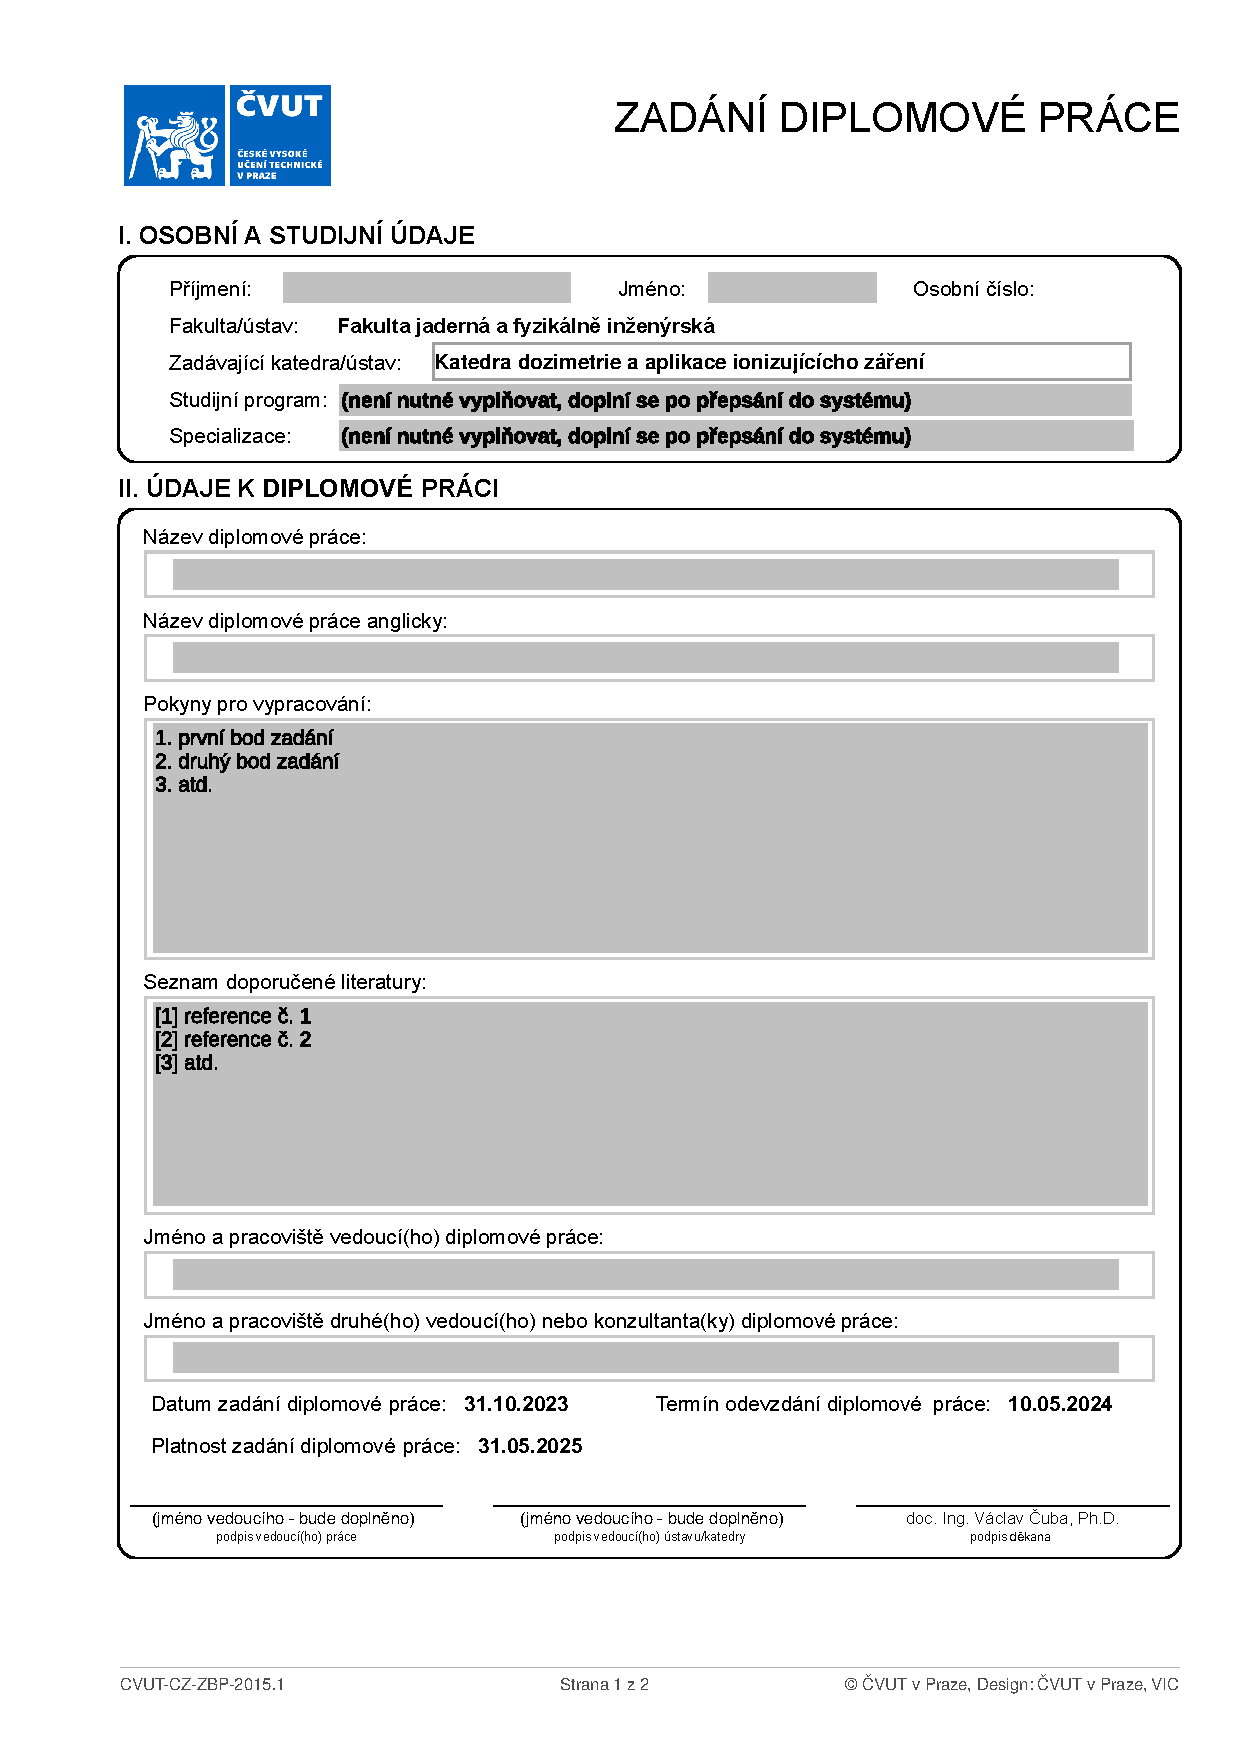
\includepdf[pages=1]{zadani.pdf}
%\includepdf[pages=2]{zadani.pdf}

\newpage 
\thispagestyle{empty}  

~ 
\vfill 

{\bf \noindent Prohlášení} 

\vspace{0.5cm} 
\noindent Prohlašuji, že jsem svoji diplomovou práci vypracovala samostatně a použil/a jsem pouze podklady uvedené v~přiloženém seznamu.

\vspace{5mm}\noindent V~Praze 1.\,8.\,2021\hfill 
    \begin{tabular}{c}                              
    ........................................\\  
    \autor                                     
    \end{tabular}                                  


\newpage
\thispagestyle{empty}

~
\vfill

{\bf \noindent Poděkování} 

\vspace{0.5cm} 
\noindent Ráda bych poděkovala\dots

Tento výzkum byl podpořen \dots

\begin{flushright}
\autor
\end{flushright} 

\newpage
\thispagestyle{empty}

{
	\setlength{\parindent}{0pt}
	
	\textit{Název práce:}
	\textbf{\nazevcz} \\
	
	\textit{Autor:} \autor \\
	
	\textit{Obor:} \obor \\
	
	\textit{Druh práce:} Diplomová práce \\
	
	\textit{Vedoucí práce:}  \vedouci, \pracoviste \\
	
	\textit{Konzultant:}  \konzultantka, \pracoviste \\ 
	
	\textit{Abstrakt:} 
	\abstrCZ \\
	
	\textit{Klíčová slova:}  \klicova
}

\newpage
\thispagestyle{empty}
{
	\setlength{\parindent}{0pt}
\textit{Title:}
\textbf{\nazeven} \\

\textit{Author:} \autor \\

\textit{Abstract:} 
\abstrEN \\

\textit{Key words:}  \keyword
}


\tableofcontents

\newpage
\chapter*{Úvod}\addcontentsline{toc}{chapter}{Úvod}

Ve Wordovském vzoru BP/DP prací KDAIZ se uvádí:
\begin{quote}
    Úvod by měl poskytovat základní informace o obsahu práce. Měl by také obsahovat vymezení tématu práce (a důvod výběru tématu), vymezení cíle/cílů práce, způsob/metodu dosažení cíle (stručný nástin práce) a předpoklady/omezení práce. Měl by být stručný a výstižný, doporučuje se postupovat od obecného ke specifickému.

    Většinou úvod zabere 1 stránku (max. 3 stránky), nerozděluje se na podkapitoly.

    Spolu se závěrem se úvod doporučuje psát až po dokončení celé práce.
\end{quote}


\chapter{Teoretický úvod}
\label{sec:teorie}

\noindent Forma závěrečné práce je popsaná na \href{ https://kdaiz.fjfi.cvut.cz/studium/bakalarske-studium/bakalarska-prace/}{stránkách KDAIZ}.

Teoretický úvod obsahuje stav problematiky. Protože úvod má být krátký, state-of-the-art část přijde až sem.

\section{Nástroje}
\label{sec:nastroje}

\noindent Nechcete-li si nic dalšího instalovat, lze práci psát v prohlížeči pomocí webového nástroje Overleaf --- tato šablona je dostupná přes následující odkaz; stačí si ji otevřít a přes \texttt{File/Make a copy} uložit kopii projektu do Vašeho účtu:

\begin{quotation}
\href{https://www.overleaf.com/read/znrvrtjfkhbg#30e8b1}{https://www.overleaf.com/read/znrvrtjfkhbg\#30e8b1}. 
\end{quotation}

Overleaf zároveň umí spolupracovat s nejrozšířenějšími systémy pro správu citací, viz \href{https://www.overleaf.com/blog/639-tip-of-the-week-overleaf-and-reference-managers}{Tip of the Week: Overleaf and Reference Managers}. 

Pokud preferujete mít vše u sebe, šablona je též k dispozici v git repozitáři na URL:

\begin{quotation}
    \href{https://github.com/vaclavstepan/kdaiz-zp-template}{https://github.com/vaclavstepan/kdaiz-zp-template}
\end{quotation}

Skvělým úvodem do použití systému \LaTeX\ je kniha pana Satrapy \LaTeX\ pro pragmatiky \cite{satrapa_latex_2011}. V \LaTeX\ je také k dispozici spousta balíčků maker zjednodušujících práci. Například nechcete-li si lámat hlavu, jak psát správně stupně Celsia,  \href{https://texdoc.org/serve/siunitx/0}{siunitx}.

K sazbě a typografii lze doporučit web \href{http://www.liteera.cz}{Litéra} (pro češtinu) a pro práce v angličtině pak Buttericks's Practical Typography~\cite{butterick_matthew_buttericks_nodate}. 
Jazyková pravidla pro práce v češtině viz.~\cite{ijp}.

Pro doplnění tvrdých mezer za jednopísmenné předložky můžete využít buď programů \href{https://petr.olsak.net/ftp/olsak/vlna/}{vlna} od \href{https://petr.olsak.net/}{Petra Olšáka}, nebo např. v AucTeX pro Emacs pomocí makra \texttt{tildify}. Vlna je také součástí distribuce TeXLive.

Budete-li chtít psát bez připojení k síti, budete potřebovat \LaTeX\ (třeba z~\href{https://tug.org/texlive/}{TeXlive}) pro překládání zdrojových souborů do PDF a nejspíš \verb?git? pro správu verzí. K~distribuované správě verzí v~\verb?git? se více dozvíte třeba v knize Scotta Chacona a Bena Strauba~\cite{chacon_pro_2014}.

\subsection{Příprava obrázků}
\label{sec:obrazky}

Pro zpracování obrázků a ilustrací by se vám mohly hodit některé z následujících volně dostupných nástrojů, podle formy a obsahu:
\begin{description}
\item[Vektorové ilustrace] --- \href{https://inkscape.org/cs/}{Inkscape}
\item[Bitmapové obrázky] --- \href{https://gimp.org/}{GIMP}
\item[Diagramy a schémata] --- \href{https://www.yworks.com/products/yed}{yEd}
\end{description}


\chapter{Materiály a metody}
\label{sec:metody}

\noindent Popis použitých metod a přístrojů, včetně příkladu tabulky  (\ref{tab:priklad}) a obrázku (\ref{fig:priklad}).

\begin{table}[hbtp]
    \centering
    \caption{Počet zvířat jednotlivých druhů na \SI{1}{\meter\squared}. Popisek je nad tabulkou.}
    \begin{tabular}{|l|r|}\hline
        zvíře & počet \\ \hline\hline
        medvědi & 8\\
        tučňáci & 17\\\hline
    \end{tabular}
    \label{tab:priklad}
\end{table}

\begin{figure}[hbtp]
    \centering
    
\includegraphics[width=0.5\textwidth]{cvut.jpg}
    \caption{Příklad lva. Popisek u obrázku je pod ním.}
    \label{fig:priklad}
\end{figure}



\chapter{Výsledky}
\label{sec:vysledky}

\noindent Tady jsou výsledky a jejich popis. Metody a přístroje použité k jejich získání jsou popsány dříve, v~kapitole (\ref{sec:metody}). Prostor na diskusi výsledků (proč to vyšlo, nevyšlo, jak to zapadá do kontextu a co by třeba bylo třeba udělat příště lépe a jinak) bude v~další kapitole (\ref{sec:diskuze}).



\chapter{Diskuze}
\label{sec:diskuze}

Inu, vyšlo nám to, ale\dots


\chapter{Závěr}
\label{sec:zaver}

\noindent Protože náhodný čtenář nejspíš nebude mít čas číst celou práci, tady shrneme, co vyšlo a jak to splňuje cíle práce. Mohou tu být odkazy zpátky do textu, ale je to celkem krátká textová část.

V závěru práce byste měli svou práci zhodnotit jako autor. Závěr by tedy měl obsahovat:
\begin{itemize}
\item shrnutí výsledků, ke kterým autor dospěl,
\item přínos autora práce k řešené problematice (co je v práci původní),
\item zhodnocení využitelnosti dosažených výsledků,
\item možné pokračování práce (resp. další náměty pro řešení v uvedené oblasti).
\item Závěr se většinou vejde na 1 stránku (max. 3 stránky).
\end{itemize}




\addcontentsline{toc}{chapter}{Literatura}
\printbibliography

%\listoftables
%\listoffigures
\end{document} 

